\chapter{The framework}

\section{Main Scenario}

The goal is to build a platform that allows a user to query for experts in a particular domain. The
platform extracts and unifies the required information from a variety of online sources and
subsequently builds a repository of user profiles. We basically want to create a framework that would function as a Google for finding experts given a certain subject.

We will use the following steps to build such a platform:

%verduidelijken dat de volgorde van deze stappen niet belangrijk is, ze zijn interchangeable

\begin{itemize}
	%Welke auteur namen ? Waar halen we die vandaan ? Conference sites ?
	\item \textbf{Seed data} We need a list of author names to start with.
	\item \textbf{Information extraction}
		\begin{itemize}
			\item Looking up personal information, ie. profiles from LinkedIn.
			\item Looking up publications, extracting title, co-authors and affiliation. The co-authors can be used as new input for further information extraction.
			\item Categorize publications by subject
		\end{itemize}
	\item \textbf{Disambiguation} Decide if there are different authors with the same name or different spellings of the same author's name which should be mapped to one author.
\end{itemize}

%Describe how we got to the architecture for the framework, show a figure of the (simplified + extensive) architecture and explain the different components.

\section{Features}

Based on the main scenario, we can identify a few key features our framework will need. A short summarization of each follows, explaining the challenges we face with our thesis. Each of these features will be discussed more deeply throughout this chapter.

%Beter verwijzen waar ze meer informatie per feature kunnen doornemen?

\subsection{Information extraction}

We need to extract information from multiple sources, which we will accomplish by using a plugin system. Each plugin is responsible for one source and will extract specific information which can be used by other plugins or other steps in our framework.

\subsection{Categorization}

In order to decide who is an expert regarding a certain subject, we will have to decide the subject of expertise of each author. A very important part of this will be in deciding the subject of the publications. The challenge is to decide this using as few information as possible, preferably by just inspecting the title, as getting access to the text of the publication itself is a whole lot more time- and resource-consuming.

\subsection{Disambiguation}

A challenging feature is the disambiguation. There are two reasons. The first is the fact that an author's name is not a unique reference for a person. There might be multiple authors with the same name, which means we have to take this into account when deciding who is an expert.

Secondly, an name might be spelled differently or changed throughout time. Examples are abbreviations, an extra family name because of a marriage or simply spelling errors.

\subsection{Dynamic}

There is a big dynamic concept tied to our thesis. People who are experts on a certain subject a decade ago, may not be as important anymore now or may have changed their subject of expertise. An interesting point of view would be to enable users to scroll through a timeline so they could see the changes themselves. This is however out of the scope of our thesis.

\section{Components / Architecture}

\begin{figure}[htbp]
	\centering
		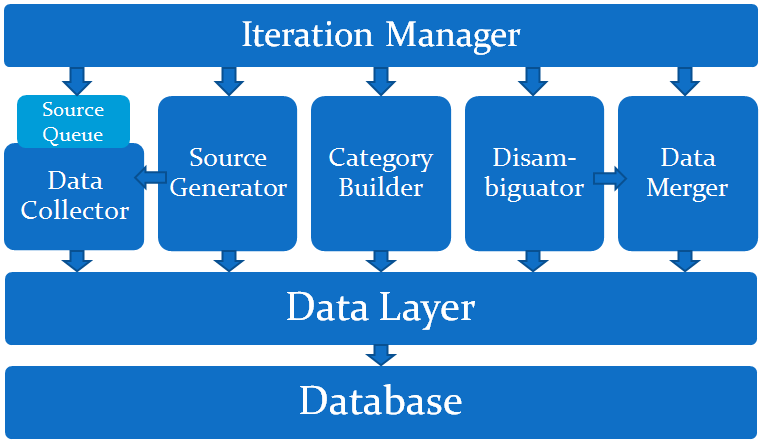
\includegraphics[width=1.00\textwidth]{fig/architectuur.png}
	\caption{First attempt at the architecture based on the necessary components}
	\label{fig:architectuur}
\end{figure}

Plugins, IterationManager, CategoryBuilder, Disambiguator, DataMerger

\section{Technologies}

\subsection{MySQL}

Discuss the differences, advantages and disadvantages between a relational datastore, a record-store and a triple-store.

\subsubsection{Relational datastore}

\subsubsection{A record-store}

\subsubsection{Triple-store}

\subsubsection{Conclusion}

We choose to use MySQL, a relational datastore, because we are familiar with it. It allows us to quickly set up our prototype to work and test our framework on.

\subsection{Two databases}

We use two databases, one for development and one for production.

The former is used to collect all information about the possible experts and their work. 

\subsection{Ruby}
